\documentclass[12pt]{report}
\usepackage{amsmath}
\usepackage{amssymb}
\usepackage{graphicx}
%\usepackage{hyperref}
\usepackage{color}
\usepackage{float}
\begin{document}
\section{Eigenvalues}\label{eigenvalues}
In this document we derive the eigenvalues of the Rouse matrix. The Rouse matrix defines the connection in the harmonic potential of the Rouse polymer. The system of differential equation governing the dynamics of the chain comprised of $N$ monomers is 
\begin{equation}
\frac{d[X(t)]}{dt}=-k[R][X(t)]+[g(t)]
\end{equation}
where the $[.]$ notation represents a matrix (vector), $[g(t)]$ is an $N$ by 1 vector of normally distributed numbers with mean 0 and STD =1, $k$ is a constant and the matrix $[R]$ is defined as:
\begin{equation}
R=\left[
\begin{matrix}
 1 & -1 &  0 &  0 &...&  &  0 \\
-1 &  2 & -1 &  0 &...&  &  0 \\
 0 & -1 &  2 & -1 &...&  &  0 \\
 . &    &    &  . &   &  &  . \\
 . &    &    &  . &   &  &  . \\
 0 &    &    &    & -1& 2& -1 \\
 0 &    &    &    &  0&-1&  1 \\     
\end{matrix}
\right]
\end{equation}

To find the eigenvalues we calculate 
\begin{equation*}
D_N=\left|[R]-\lambda[I]\right|=0
\end{equation*}
which gives us a matrix of the form 
\begin{equation*}
R=\left[
\begin{matrix}
 y & -1 &  0 &  0 &...&  &  0 \\
-1 &  x & -1 &  0 &...&  &  0 \\
 0 & -1 &  x & -1 &...&  &  0 \\
 . &    &    &  . &   &  &  . \\
 . &    &    &  . &   &  &  . \\
 0 &    &    &    & -1& x& -1 \\
 0 &    &    &    &  0&-1&  y \\     
\end{matrix}
\right]
\end{equation*}
with $x=2-\lambda$, and $y=x-1$.

Developing the determinant by the last column we find a recursion relation as follows 
\begin{equation*}
D_N = yD_{N-1}-D_{N-2}
\end{equation*}

since the recursion relation is slightly different for $D_{N-1}$, bt remains the same for all $j\leq N-1$, we solve the recursion relation for $D_{N-1}$ and then return to define the last term $D_N$ using the relation above. 

The recurrence relation is:
\begin{equation*}
D_z = xD_{z-1}-D_{z-2}
\end{equation*}

with the boundary conditions
\begin{equation*}
D_1 = y 
\end{equation*}
\begin{equation*}
D_2 = xy-1
\end{equation*}
We note that according to the Rouse matrix $x=y+1$.

The particular solution to the recursion relation is 
\begin{equation*}
D_z=e^{iz\theta}
\end{equation*}

substituting it into the recursion relation gives
\begin{equation*}
e^{iz\theta}=xe^{i(z-1)\theta}-e^{i(z-2)\theta}
\end{equation*}

hence
\begin{equation*}
x=2cos(\theta)
\end{equation*}

The general solution can then be defined as 
\begin{equation*}
D_z=Ae^{iz\theta}+Be^{-iz\theta}
\end{equation*}
where $A$ and $B$ are some constants to be defined.

 Using the boundary conditions we get 
 \begin{equation*}
 y = Ae^{i\theta}+Be^{-i\theta}
 \end{equation*}
 \begin{equation*}
 A=\frac{y-Be^{-i\theta}}{e^{i\theta}}=(2\cos(\theta)-1)e^{-i\theta}-Be^{-2i\theta} =\frac{1-e^{i\theta}}{e^{-i\theta}-e^{i\theta}}=e^{i\theta/2}\frac{e^{-i\theta/2}-e^{i\theta/2}}{-2i\sin(\theta)}=\frac{e^{i\theta/2}}{2\cos(\theta/2)}
 \end{equation*}
 and 
 \begin{equation*}
 B=\frac{e^{-i\theta}-1}{e^{-i\theta}-e^{i\theta}}=\frac{e^{-i\theta/2}}{2cos(\theta/2)}
 \end{equation*}
The general solution is now
\begin{equation}
D_z=\frac{e^{i\theta/2}}{2\cos(\theta/2)}e^{iz\theta}+\frac{e^{-i\theta/2}}{2\cos(\theta/2)}e^{-iz\theta}=\frac{\cos((z+1/2)\theta)}{\cos(\theta/2)}
\end{equation}
Since the determinant must vanish, we have 
\begin{equation*}
D_N = yD_{N-1}-D_{N-2}=0
\end{equation*}
substituting the expressions for $D_{N-1}$ and $D_{N-2}$ into the equation above yields 
\begin{equation*}
yD_{N-1}-D_{N-2} = D_1D_{N-1}-D_{N-2} = 
\end{equation*}
\begin{equation*}
\frac{\cos(3\theta/2)}{\cos(\theta/2)}\frac{\cos((N-1/2)\theta)}{\cos(\theta/2)}-\frac{\cos((N-3/2)\theta)}{\cos(\theta/2)}=0
\end{equation*}
therefore 
\begin{equation*}
\cos(3\theta/2)\cos((N-1/2)\theta)=\cos((N-3/2)\theta)\cos(\theta/2)
\end{equation*}
displaying the trigonometric functions as sum of exponentials we can get
\begin{equation*}
\cos((N+1)\theta)-\cos((N-1)\theta)=0
\end{equation*}
which gives 
\begin{equation*}
-2\sin(N\theta)\sin(\theta)=0
\end{equation*}
therefore 
\begin{equation*}
\theta = \frac{p\pi}{N}
\end{equation*}
$p=0,1...,N-1$ (since we have $N$ solutions)\\

The eigenvalues are then
\begin{equation*}
\lambda_p=2-x = 2-2\cos(\theta_p)=2\left(1-\cos(\frac{p\pi}{N})\right)=4\sin^2(\frac{p\pi}{2N})
\end{equation*}
$p=0,1,...,(N-1)$.

\section{Eigenvectors}
the $k^{th}$ entry in the $p^{th}$ eigenvector is 

\begin{equation*}
c_k = \sqrt{\frac{2}{N}}\sin(\frac{k\pi p}{N})
\end{equation*}

with $k=1,2,..,N$ and $p=0,1,...N-1$

\section{Eigenvalues of a ring of beads}
connecting bead 1 and $N$ to form a ring, we now search for the eigenvalues of the system. We have to find the determinant of the matrix
\begin{equation*}
D_N=|R-\lambda I|=\left|
\begin{matrix}
 x  & -1 &  0 &  0 &...&  & -1 \\
-1  &  x & -1 &  0 &...&  &  0 \\
 0  & -1 &  x & -1 &...&  &  0 \\
 .  &    &    &  . &   &  &  . \\
  .  &    &    &  . &   &  &  . \\
 .  &    &    &  -1 &  x &-1  &  0 \\
 0  &    &    &    & -1& x& -1 \\
 -1 &    &    &    &  0&-1&  x \\     
\end{matrix}
\right|
\end{equation*}

with $x=2-\lambda$. We can apply to the matrix of size $(N-1)\times (N-1)$ the same procedure as before and try to solve it recursively. The boundary conditions now read
\begin{equation*}
D_1 = x; D_2 = x^2-1
\end{equation*}
According to the solution in section \ref{eigenvalues} and in \cite{lin2011polymer}, we have 
\begin{equation*}
D_{N-1}= \frac{\sin(N\theta)}{\sin(\theta)}
\end{equation*}

The relationship between $D_N$ and $D_{N-1}$ is found by developing the determinant of $D_N$ according to the last column
\begin{eqnarray*}
D_N &=& x(-1)^{2N}D_{N-1}+(-1)(-1)^{2N-1}[D_{N-2}+1]+(-1)^{N+2}[(-1)^{3(N-1)}+(-1)^{N+1}D_{N-2}]\\
    &=& xD_{N-1}+D_{N-2}[1+(-1)^{2N+3}]+1+(-1)^{4N-1}\\
    &=& xD_{N-1}=2\cos(\theta)D_{N-1}=2\cos(\theta)\frac{\sin(N\theta)}{\sin(\theta)}=2\cot(\theta)\sin(N\theta)=0
\end{eqnarray*}
$D_N$ is periodic with a period of $\pi$. A characteristic plot of $D_10$ is shown in the Figure \ref{determinantOfaRouseRingWith10Beads}
\begin{figure}[H]
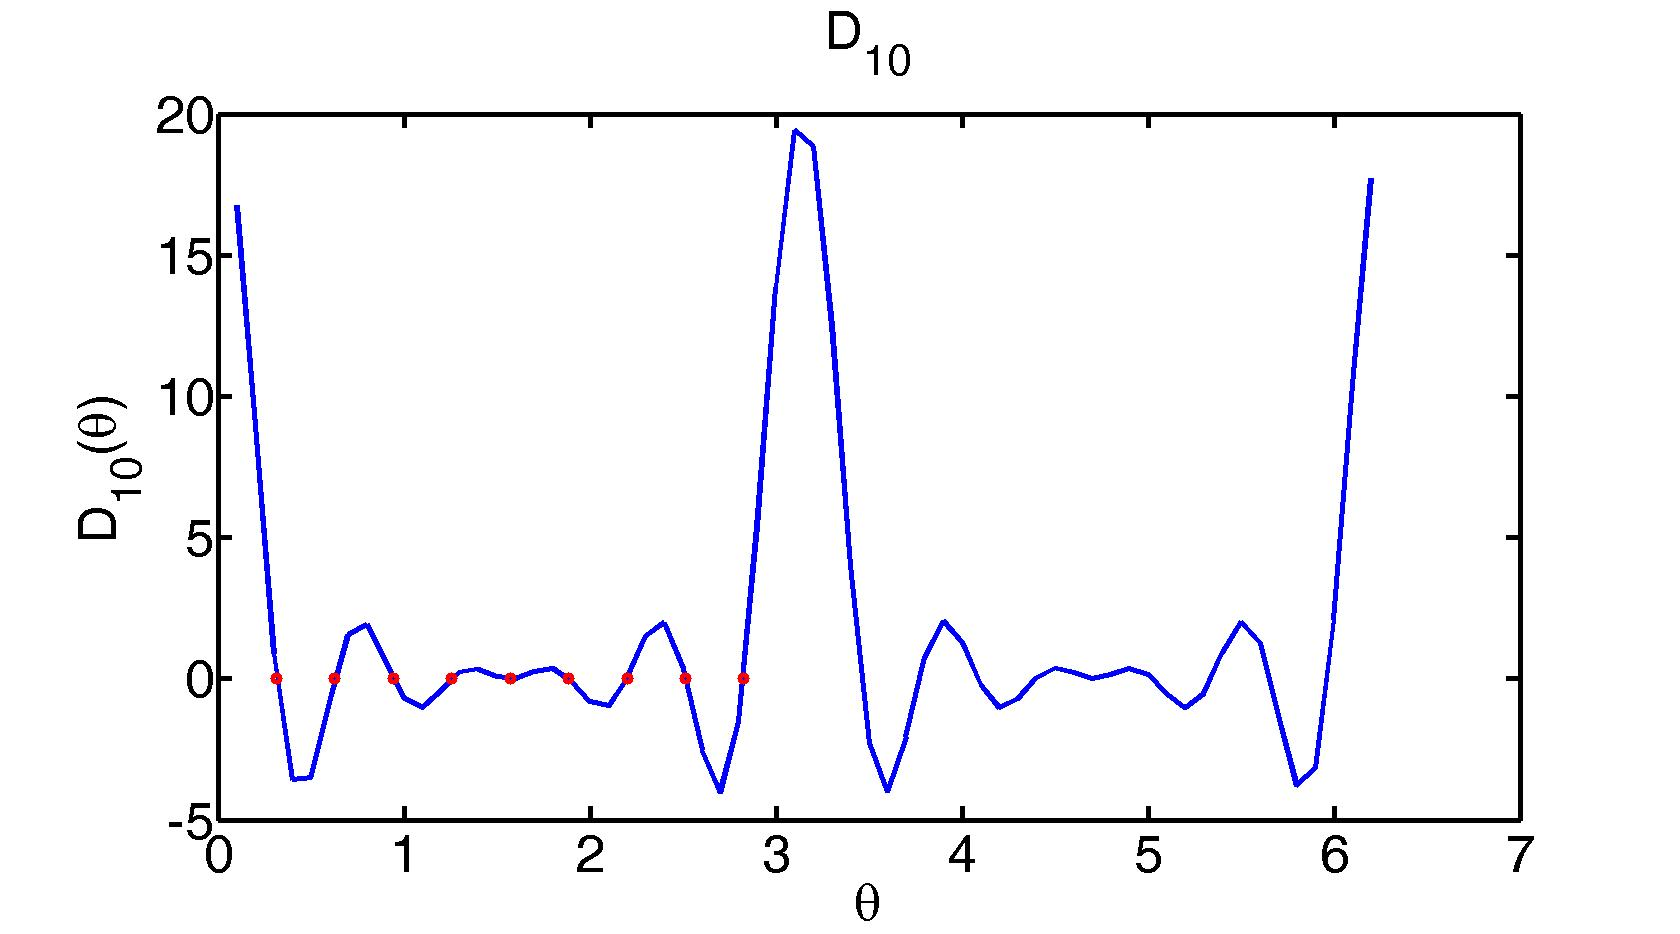
\includegraphics[scale=0.2]{determinantOfaRouseRingWith10Beads}
\caption{A plot of the determinant $D_{10}$ of a Rouse chain with 10 beads, when bead 1 and 10 are connected to form a loop. $\theta$ ranges from o to $2\pi$. The first 10 zeros of the determinant are shown in red circles}\label{determinantOfaRouseRingWith10Beads}
\end{figure}
For $p=1,2,...,N$ we have 
\begin{equation*}
\theta = \frac{\pi p}{N},
\end{equation*}
to zero out the term $\sin(N\theta)$ and 
\begin{equation*}
\theta = p\pi
\end{equation*}
to zero out $\cot(\theta)$. From $2-\lambda=2\cos(\theta)$, we get $\lambda = 2(1-\cos(\theta))$. Substituting the values for $\theta$ we have
\begin{equation*}
\lambda(p) = 2(1-\cos(\frac{\pi p}{N}))
\end{equation*} 



  
% Bibliography  
\bibliographystyle{plain}
\bibliography{EigenvaluesAndEigenvectorsOfTheRouseMatrixBibliography} % the bibliography.bib
\end{document}